A Internet tem início em meados de 1969, como ARPANET em uma pesquisa financiada pela \acrfull{DARPA}, uma agência \acrfull{DoD} dos Estados Unidos da América. No final desse ano a ARPANET foi lançada e conectava quatro universidades, em 1973 a primeira conexão internacional da ARPANET foi feita. Em 1982 o conceito de Internet começou a surgir, junto com ele novos protocolos surgiram para padronizar a comunicação entre essa redes como os protocolos IP e TCP, que continuam sendo os protocolos base da Internet até hoje \cite{Lipson2002TrackingAT}.

Essa tecnologia revolucionou a troca de informações, transformando em algo fácil, rápido e eficiente, pavimentando o caminho para a sociedade globalizada e estando hoje presente em ambientes essenciais que uma nação necessita. Outra grande revolução que a internet trouxe para a sociedade pós-moderna foi a criação de um novo ambiente de conflito. Antes de seu surgimento os conflitos se passavam apenas na esfera física, onde grande movimentações do inimigo podem ser descobertas possibilitando movimentos de antecipação e além disso evidencias físicas podem ser deixadas possibilitando seu rastreio e talvez sua captura. Com o surgimento da internet os conflitos passaram a existir também na esfera digital, que é um ambiente sem fronteiras, com maior anonimato e a um custo muito menor que um conflito na esfera física.  Os ataques que ocorrem em conflitos na esfera digital são denominados como ciberataques.

Apesar da internet criar essa nova esfera de conflito não é nela que reside o perigo dos ciberataques, a maior ameaça está na enorme quantidade de dispositivos vulneráveis conectados a ela. Novas vulnerabilidades em softwares executados por esses dispositivos são sempre descobertas, e uma vez apresentada ao público podem vir a comprometer uma imensa quantidade de dispositivos \cite{Lipson2002TrackingAT}. Outro fator importante é que a sofisticação dos ciberataques tem crescido enquanto a expertise necessária para executa-los tem diminuído, isso é explicado com o advento de ferramentas para a preparação, gerenciamento e execução desses ataques. A figura \ref{img:ExpVSSof} apresenta essa sofisticação dos ciberataques pela expertise do atacante.

\begin{figure}[H]
     \centering
     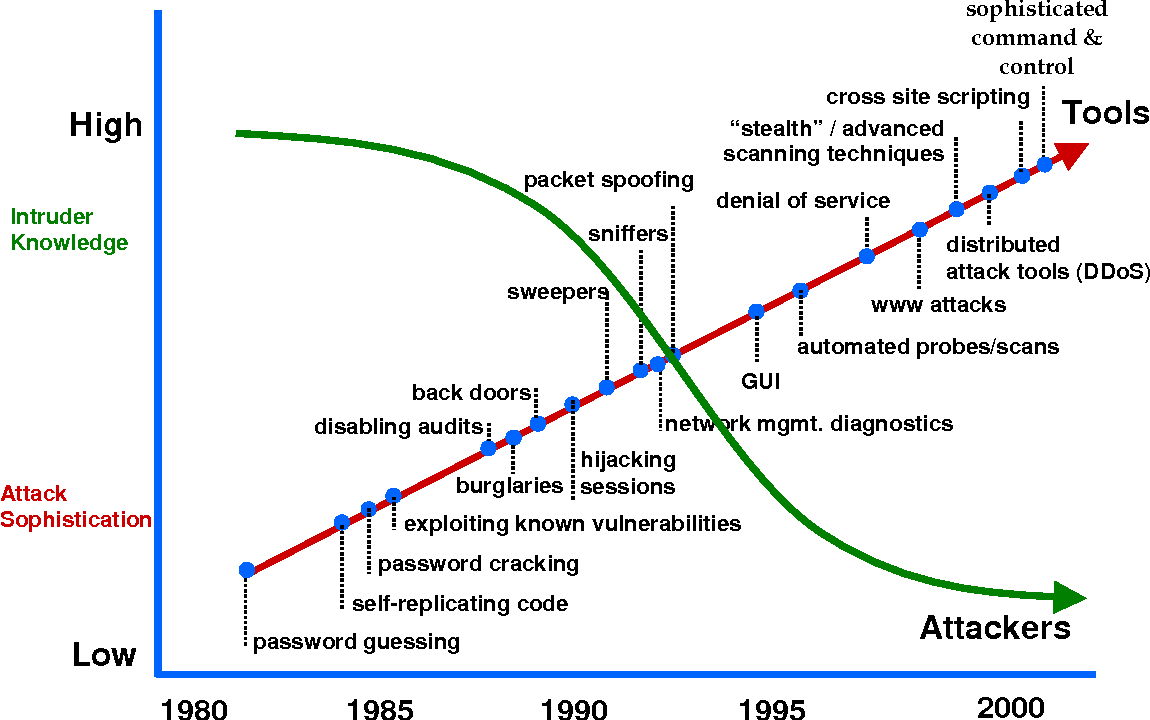
\includegraphics[scale=0.35]{img/24-Figure1-1.png}
     \caption{ Sofisticação do ataque pela expertise do atacante \cite{Lipson2002TrackingAT} }
     \label{img:ExpVSSof}
\end{figure}

As motivações para se efetuar um ataque na esfera digital não difere das motivações de ataques na esfera física, sendo eles políticos, econômicos e socio-culturais \cite{Gandhi2011}.

Com toda essa disponibilidade e facilidade para a execução de ciberataques somadas à dependência da internet que se tem hoje, se tornou algo rotineiro a ocorrência de ciberataques em todo o mundo. 

\section{Motivação}

Com toda essa dependência que se tem atualmente da internet na troca de informações para a tomada de decisão era inevitável o surgimento de ataques que bloqueassem os serviços disponibilizados por ela. Um ciberataque amplamente utilizada para cumprir esse objetivo é o ataque de negação de serviço.

Esse ataque consiste em esgotar os recursos de uma máquina ou infraestrutura , impedindo que a vítima consiga disponibilizar seus serviços na rede ou acessar outros. Para efetuar o ataque o atacante pode utilizar uma única fonte ou distribuir o trabalho em várias fontes para aumentar o seu poder computacional e aumentar o seu anonimato e transformando o ataque em uma ataque de negação de serviço distribuído. 

Esse tipo de ataque não possui uma dificuldade muito alta para sua implementação, entretanto ele pode causar um grande estrago, podem trazer prejuízos enormes a uma pessoa, empresa ou nação a um custo muito baixo.

\section{Justificativa}

No dia 28 de fevereiro de 2018 o serviço do Github ficou inoperante das 17:21 às 17:26 UTC e intermitentemente indisponível das 17:26 às  17:30 UTC devido a um ataque de negação de serviço distribuído que alcançou um pico de 1.35Tbps enviando 126.9 milhões de pacotes por segundo. O serviço disponibilizado por eles é utilizado no mundo inteiro por varias pessoas e empresas, com sua disponibilidade sendo de crítica importância para seus usuários \cite{GitHubDDoS}.

Quatro dias depois foi registrado pela Arbor Network a mitigação de um outro ataque a uma empresa norte-americana não divulgada que chegou a um pico de 1.7Tbps, sendo o maior ataque de negação de serviço registrado até hoje \cite{LiamDDoS} \cite{cloudflareDDoS}.

Esses dois incidentes utilizaram servidores Memcached expostos a internet como refletores/amplificadores para efetuar o ataque e nos mostram o estrago que tal ataque pode fazer, com muitas vezes o atacante pedindo um pagamento para cessar o ataque.

\section{Objetivos}

O objetivo da monografia é desenvolver uma ferramenta que sirva como uma plataforma para a implementação de ataques de negação de serviço para viabilizar uma análise do Memcached como um refletor em um ataque de negação de serviço.

A ferramenta desenvolvida irá facilitar a implementação de futuros ataques evitando o retrabalho na implementação de um injetor de pacotes e de uma \acrfull{CLI}. O desenvolvedor irá se preocupar em desenvolver apenas o mirror para o seu ataque e fazer pequenas alterações no código da ferramenta para inclui-lo.

Vale ressaltar que esse trabalho possui apenas fins acadêmicos, com o autor e seu orientador não se responsabilizando por qualquer uso inapropriado da ferramenta cujo código se encontra sob guarda do autor e seu orientador.

\section{Organização do texto}

Esse trabalho está organizado na seguinte forma:

\begin{itemize}
\item O capítulo 2 aborda o fundamento teórico necessário para o entendimento do trabalho;
\item O capítulo 3 apresenta a ferramenta desenvolvida;
\item O capítulo 4 apresenta os dados obtidos em laboratório e a análise desses dados;
\item O capítulo 5 apresenta a conclusão e as propostas para trabalhos futuros.
\end{itemize}




